\chapter{Amazon Kindle Fire Development}
\label{appendix-kindle-fire-development}

\textbf{Amazon Development}

\href{https://developer.amazon.com/apps-and-games}{Why developers are choosing Amazon Appstore}

\url{https://developer.amazon.com/dashboard}

\begin{figure}
    \centering
    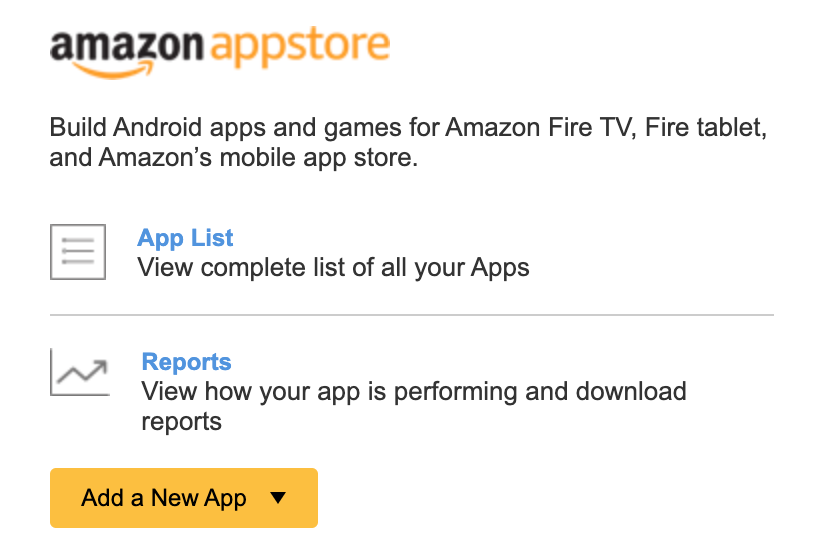
\includegraphics{images/amazonappstore/ad-app-list-reports-2021-01-07.png}
    \caption{Amazonappstore App List and Reports}
    \label{fig:amazonappstore-app-list-reports}
\end{figure}

\begin{figure}
    \centering
    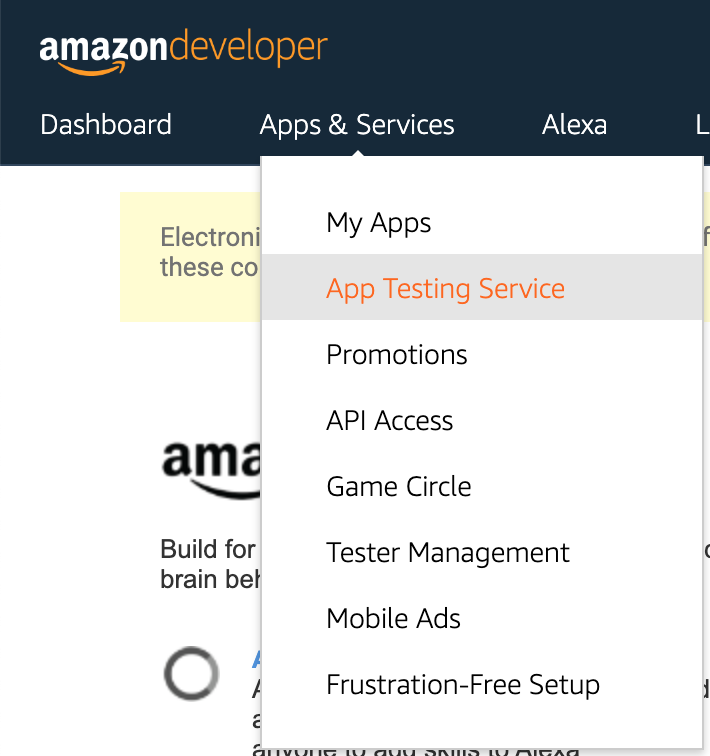
\includegraphics{images/amazonappstore/ad-apps-and-services-2021-01-07.png}
    \caption{Amazonappstore Apps \& Services}
    \label{fig:amazonappstore-apps-and-services}
\end{figure}

Amazon Mobile Analytics is now Amazon Pinpoint

Collect, View and Export App Analytics
Mobile Analytics is now part of Amazon Pinpoint

All the functionality that was previously part Amazon Mobile Analytics is now included in our Amazon Pinpoint service. Just like Mobile Analytics, Pinpoint lets you measure app usage and revenue. In addition, Pinpoint extends this capability by making it easy to run targeted campaigns to drive user engagement in mobile apps. Amazon Pinpoint helps you understand user behavior, define which users to target, determine which messages to send, schedule the best time to deliver the messages, and then track the results of your campaign. If you are a previous Mobile Analytics customer, we encourage you try Amazon Pinpoint.

\url{https://aws.amazon.com/mobileanalytics/}

\begin{comment}
Stuff to write up here or in the discussion section 
https://support.magplus.com/hc/en-us/articles/203808178-Android-Kindle-Fire-Building-an-App-Step-by-Step | Android/Kindle Fire - Building an App Step-by-Step – Mag+ Designd Support
https://developer.amazon.com/docs/fire-tablets/ft-create-your-first-kindle-fire-app.html | Create Your First App (Fire Tablets) | Fire Tablets
https://developer.amazon.com/dashboard | Amazon Apps & Services Developer Portal
https://aws.amazon.com/mobileanalytics/ | AWS | Amazon Mobile Analytics - Mobile App Analytics
https://developer.amazon.com/apps-and-games | App and Game Development | Amazon Appstore Developer Portal
https://developer.amazon.com/docs/app-submission/migrate-existing-app.html | Migrating An Existing App to the Amazon Appstore | App Submission and Testing
https://docs.amplify.aws/lib/analytics/getting-started/q/platform/android#record-events | Analytics - Getting started - Amplify Docs
https://developer.amazon.com/docs/fire-tablets/ft-data-transfers-and-mobile-networks.html | Data Transfers and Mobile Networks (Fire Tablets) | Fire Tablets
https://developer.amazon.com/docs/apps-and-games/sdk-downloads.html | SDK Downloads | Appstore
https://developer.amazon.com/documentation | Technical Documentation | Amazon Developer Portal
https://developer.amazon.com/docs/app-submission/presubmission-checklist.html | Amazon Appstore Presubmission Checklist | App Submission and Testing
https://support.magplus.com/hc/en-us/articles/204274108-Kindle-Fire-Creating-an-App-in-the-Amazon-Developer-Console | Kindle Fire - Creating an App in the Amazon Developer Console – Mag+ Designd Support
https://support.magplus.com/hc/en-us/articles/203808228-Reference-Mag-Analytics-101 | Reference - mag+ Analytics 101 – Mag+ Designd Support
https://www.mobileatscale.com/ | Mobile Apps at Scale: 33 Engineering Challenges
\end{comment}